\caption{Table \ref{det_main_all_B_p3.5}, \ref{det_main_all_C_p3.5}, \ref{det_all_all_B_p3.5} and \ref{det_all_all_C_p3.5} are showing the detail slowdowns added to the code by each phase of ParLOT(main and all) for input sizes of \textit{B} and \textit{C}. I put my observations of all four tables over here. I can integrate all of these four tables into one (something like table \ref{genDet_B_p3.5}) (Your opinion). \textbf{npin} is just the slowdown caused by initializing Pin's routines on top of the target application without doing anything else (no instrumentation, tracing, compression and I/O.  \textbf{dpin} is almost identical to ParLOT except it stores the generated compressed traces to "/dev/null". The purpose of \textit{dpin} is to see how much of the overall overhead is because of I/O and data-related slowdowns. In \textbf{wpin}, and all collected data would be stored as is to the disk. The results of this tools shows how much efficiency our compression approach adds to ParLOT. Last row of tables shows geometric mean of each of its above values showing how much each phase of ParLOT slows down the native execution. In general, we all expect that the slowdowns of $npin < dpin < ParLOT < wpin $. But majority of numbers are not like that. For larger input sizes (tables \ref{det_all_all_C_p3.5} and \ref{det_main_all_C_p3.5}) and also for for ParLOT(all) (tables \ref{det_all_all_B_p3.5} and \ref{det_all_all_C_p3.5}) the GeoMean row numbers make more sense. I double checked the results of CHPC and Stampede and the patterns are kind of identical.  In most of the table entries (in particular for smaller number of cores), the differences between the average slowdown of \textit{dpin} and \textit{ParLOT} is very insignificant which shows that ParLOT is not an I/O-bounded tool. One of the problems that I had and still have is running \textit{wpin} on input \textit{C}. I did not have the results of \textit{wpin} on \textit{C} input. While I was preparing these tables and I felt secure about not wasting SUs, I let \textit{wpin} run on \textit{C} input. Unfortunately, most of the experiments crashed due to a \textit{PMPI} error so the results are unreliable. That is why I put 0 in table \ref{det_main_all_C_p3.5} and \ref{det_all_all_C_p3.5} under \textit{wpin}. Figures \ref{chartDet_B_wc_byTool_p3_5}, \ref{chartDet_B_woc_byTool_p3_5} and \ref{chartDet_C_wc_byTool_p3_5} visualize numbers from these tables.} 


\begin{figure*}[!t]
\centering
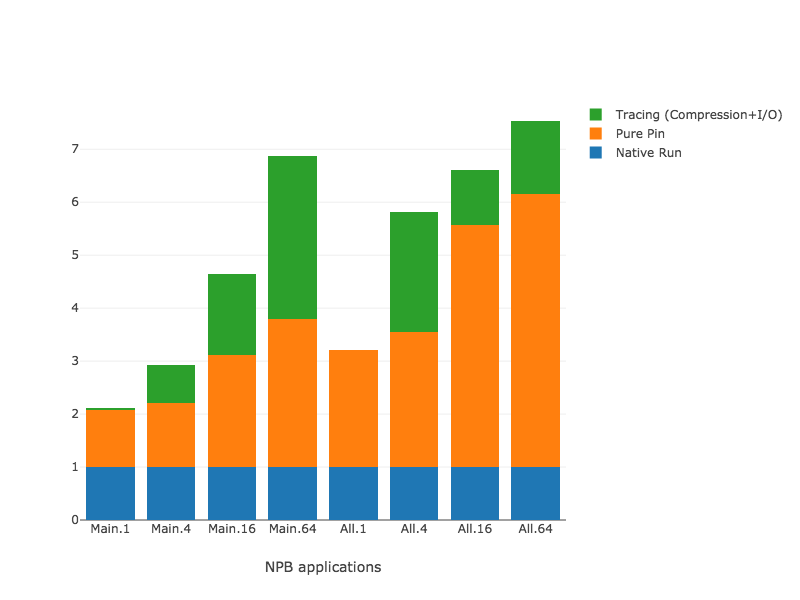
\includegraphics[width=5in]{figs.psc/chartDet_B_wc_byTool_p3_5.png}
\caption{ Input size: \textbf{B}. Each bar is stacked value of slowdowns : $Native Run = 1$ , $Pure Pin = npin - 1$ , $Tracing = ParLOT - npin$. Label of each bar is, (main/all).(1/4/16/64). This graph shows why ParLOT does not scale that well. The overhead that Pin itself is adding to the native run is growing with higher number of cores. The green part of each bar (tracing) is the overhead that our approach is adding. Fig \ref{chartDet_B_woc_byTool_p3_5} shows the effectiveness of our compression approach}
\label{chartDet_B_wc_byTool_p3_5}
\end{figure*}


\begin{figure*}[!t]
\centering
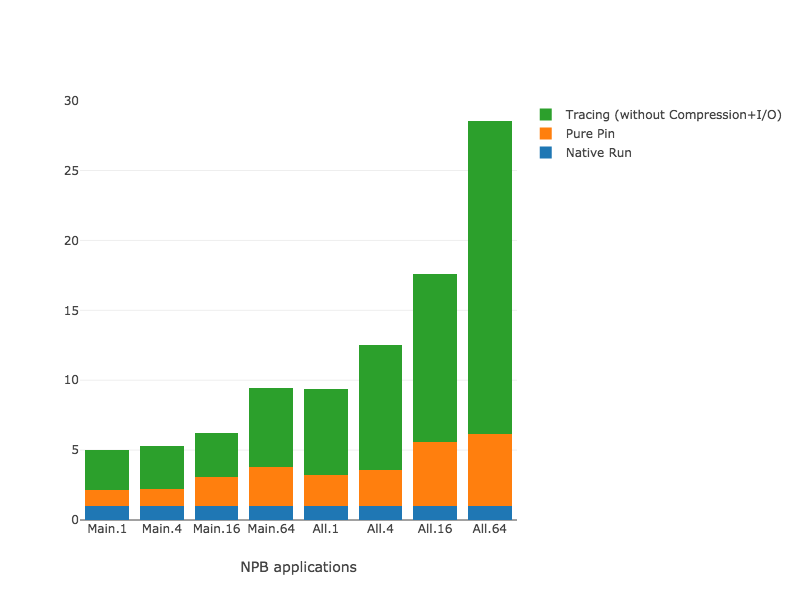
\includegraphics[width=5in]{figs.psc/chartDet_B_woc_byTool_p3_5.png}
\caption{ Input size: \textbf{B}. Each bar is stacked value of slowdowns : $Native Run = 1$ , $Pure Pin = npin - 1$ , $Tracing (w/o \_compression) = wpin - npin$.
This graph clearly shows how much impact our compression method has on the performance of ParLOT.
}
\label{chartDet_B_woc_byTool_p3_5}
\end{figure*}


\begin{figure*}[!t]
\centering
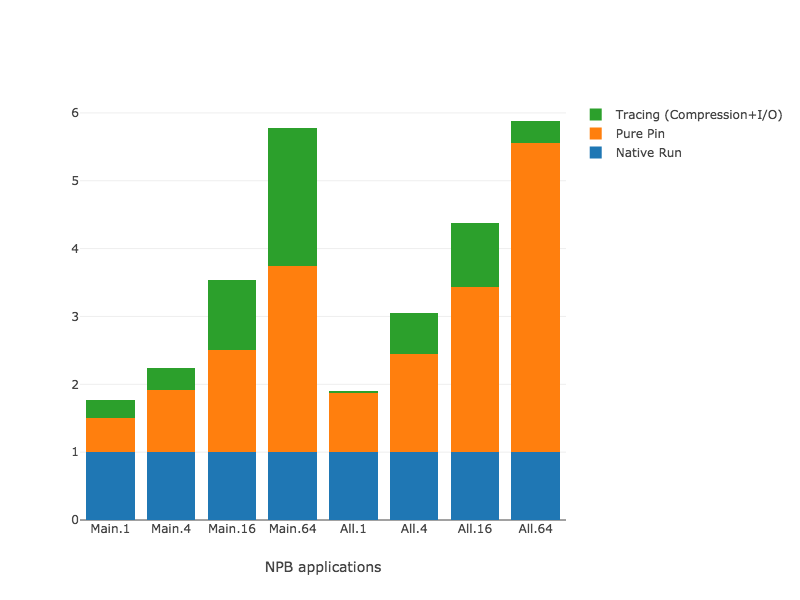
\includegraphics[width=5in]{figs.psc/chartDet_C_wc_byTool_p3_5.png}
\caption{Input size: \textbf{C}. This chart is similar to fig \ref{chartDet_B_wc_byTool_p3_5} but for larger input size C. As I mentioned in the table description, ParLOT seem to have better performance on larger input sizes. General shape of this chart matches fig \ref{chartDet_B_wc_byTool_p3_5} which shows the deterministic behavior of our tool and application.}
\label{chartDet_C_wc_byTool_p3_5}
\end{figure*}